\chapter{On the meaning of geodesics}
\textit{\today\newline
Jan Střeleček\newline}


\section{Transport using quenches}
\label{sec:quenches}
Unifying the ground states $\ket{o(\llambda)}$ over all points $\llambda\in\R^n$ in the parameter space, we get the ground state manifold. Here the fidelity $f$ and distance $s$ are defined
\begin{equation}
    \d s^2 \equiv 1-f^2\equiv 1-\left|\braket{o(\bm\llambda+\delta\bm\llambda)|o(\bm\llambda)}\right|^2.
    \label{eq:distanceOnM0}
\end{equation}

The final fidelity of transport on $\M$ is then
\begin{equation}
    F=\iint g_{\mu\nu}\d\lambda^\mu\d\lambda^\nu = \int_{t_i}^{t_f}\underbrace{\int_{t_i}^\tau g_{\mu\nu}\der{\lambda^\mu}{t}\der{\lambda^\nu}{t} \d t}_{\mathcal{L}(\lambda^\mu,\dot\lambda^\mu,\tau)}\d \tau .
\end{equation}
Using Euler-Lagrange equations for time-independent $g_{\mu\nu}=g_{\mu\nu}(\lambda^\mu)$, leads to
\begin{equation}
    \int_{t_i}^{\tau}\left[g_{\mu\nu,\kappa}\dot\lambda^\mu\dot\lambda^\nu - \der{}{t}\left[g_{\mu\nu}\left(\delta^\mu_\kappa\dot\lambda^\nu+\dot\lambda^\mu\delta^\nu_\kappa\right)\right]\right]\d t=0,
\end{equation}
which needs to be zero for integration over any subset $(t_i,\tau)$ leads to a zero condition for the integrand itself, which leads to the geodesic equation.

This means that the geodesic should \emph{maximize the fidelity of the transport} between two points. One needs to stop for a while and realize what is the physical meaning of this transport. What the system at any point in the parameter space sees is how far away are all points in his surrounding. In the case of a geodesic, the direction of the smallest distance is then chosen, and the procedure repeats. The problem is that moving in the direction $\delta\llambda$ means physically changing the eigenstate to the new one, meaning one needs to project it to the newly diagonalized system at the point $\llambda+\delta\llambda$ leading to a transition amplitude
$$A_k=\braket{o(\bm\llambda+\delta\bm\llambda)|i(\bm\llambda)}.$$
Next, we ignore higher states and continue only with the ground state. In the end, we calculate what fraction of states we can get to the final ground state, which is the probability of this event. 
 
If we imagine $\delta\llambda$ to be finite (not infinitely small, as the notation suggests), the \textbf{transport} means \textbf{doing a sequence of quenches and measuring the system after every quench}.


Some notion of the space of our Hamiltonian can be seen by quenching from $(\lambda_i;\chi_i)=(0;0)$ to $(\lambda;\chi)$, as can be seen in Figure \ref{fig:quenchFidelityFrom00}.

In Figure \ref{fig:equidistantPointsOnPath} are marked equidistant points, meaning $\int_a^b \d s=\text{some const}$ between every two neighboring points on curve. This means that if the system is measured periodically, the quenches jump smaller distances when closer to a singularity.

Decreasing time step $\Delta t$ has no effect on the relative fidelity of quenches during the evolution but has an effect on their magnitude. As one would expect, when $\Delta t\rightarrow 0$, the transport becomes adiabatic, and the fidelity at any time will become zero. This can be observed in Figure \ref{fig:plotsFidelityQuenches}, such that the shape of the point-like paths looks similar in the columns, and their magnitude decreases.

\begin{figure}[H]
    \centering
    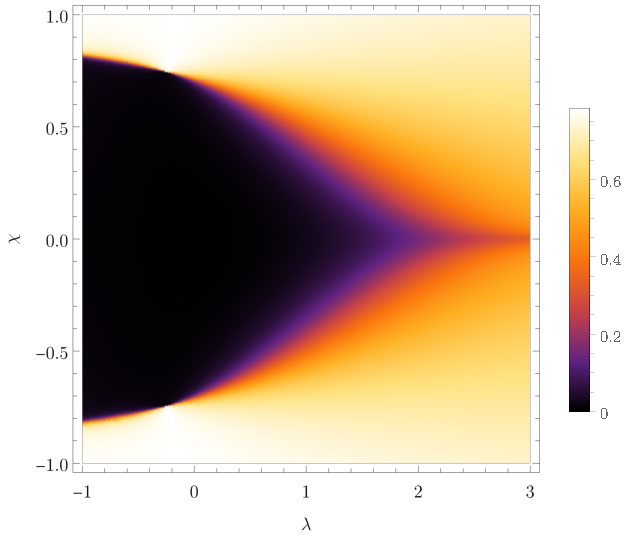
\includegraphics[scale=1.2]{../img/quenchFidelityFrom00.pdf}
    \caption{Arctangens of the fidelity of quenches from $(\lambda_i;\chi_i)=(0;0)$ to $(\lambda;\chi)$.}
    \label{fig:quenchFidelityFrom00}    
\end{figure}

\begin{figure}[H]
    \centering
    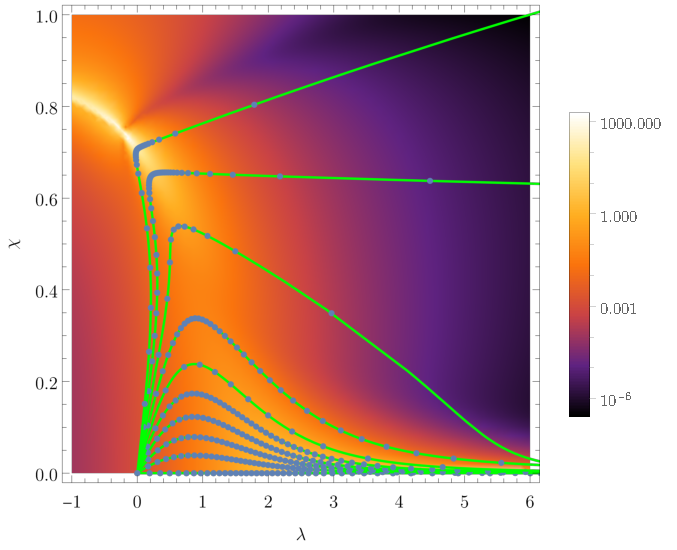
\includegraphics[scale=1.2]{../img/equidistantPointsOnPath.pdf}
    \caption{Equidistant points on geodesics of the ground state manifold.}
    \label{fig:equidistantPointsOnPath}    
\end{figure}

\begin{figure}[H]
    \centering
    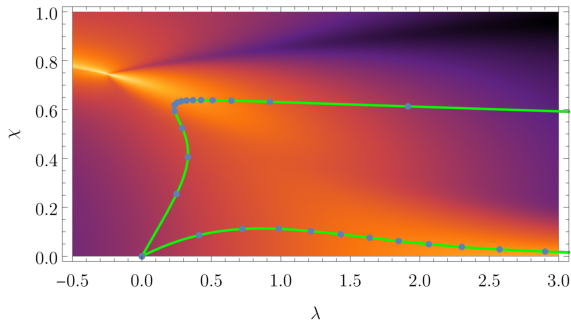
\includegraphics[scale=1.2]{../img/bg123.pdf}
    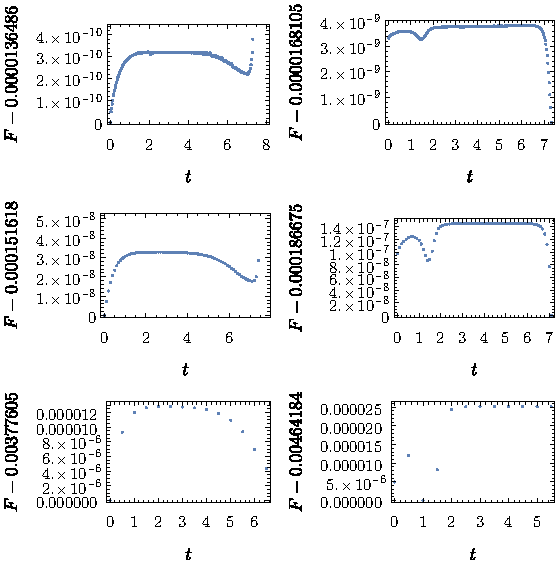
\includegraphics[scale=1.3]{../img/plotsFidelityQuenches.pdf}
    \caption{Fidelity for sequential quenches along geodesics (see green lines on top). Left (right) column corresponds to lower (upper) geodesic. Time steps from top are $\Delta t\in \{0.03,0.1,0.5\}$. Time difference between points in the plot on top is $\Delta t=0.5$.}
    \label{fig:plotsFidelityQuenches}    
\end{figure}

\chapter{Metric tensor of the higher state manifold}
Definition of the k-state manifold is
\begin{equation}
    g_{\mu\nu}^{(k)} = \Re \sum_{j\neq k}\frac{\braket{k|\pder{\HH(\llambda)}{\lambda^\mu}|j}\braket{j|\pder{\HH(\llambda)}{\lambda^\nu}|k}}{(E_k-E_j)^2}.
    \label{eq:metrictensork}
\end{equation}
One has to see it as a measure between the quantum states. The states are further away from each other when they are "more perpendicular" because the transition probability between the states is lower. The only difference here is that one state needs to be evolved using the derivative of Hamiltonian. From this goes that \emph{minimizing the distance on path} means \emph{going through the least excitation probability path}.

When one assumes a pure ground state at every point of transport, the situation using quenches, see section \ref{sec:quenches}, is reconstructed. During some general transport, in which a superposition of states is allowed, one also needs to minimize the flow of probability from higher states to even higher states and maximize the flow from higher states to lower ones. Let us try to construct a new metric tensor, which will count in those \emph{higher-state transition} effects.

\section{Higher state transition metric operator}
Imagine a driving 
\begin{align*}
    \gamma:\R &\rightarrow \R^n \\
    t &\mapsto \llambda\equiv (\lambda_1,\dots \lambda_n)
\end{align*}
This function translates the driving parameter $t$ to coordinates for Hamiltonian $\HH(\llambda)$. Assume the states
\begin{equation}
    \textcolor{purple}{\ket{\Psi(t)}=\sum_m a_m(t)\ket{m(t)}}
\end{equation}
for eigenstates $\ket{m(t)}$ of the Hamiltonian $\HH$. Now we can form a linear combination of effects on this wavefunction, where every excitation probability needs to be minimized and every deexcitation maximized. \textbf{Because $\partial_\mu \HH$ is a hermitian operator, the excitation and deexcitation will occur with the same probability. Plus if we assume the Fidelity to be $F>0.5$}, we can neglect the deexcitation probabilities and instead \textcolor{blue}{minimize only the excitations}, which can be done by introducing \emph{Higher state transition metric operator}, let's call it just the \emph{metric operator}\footnote{It's not a tensor, because it does not transform like a tensor. It depends on a path.}
\begin{equation}
    \begin{split}
        G_{\mu\nu}^{\textcolor{purple}{\psi}(t)} =& \Re \sum\limits_{j=0}^n \textcolor{blue}{\sum_{m=j+1}^n}\textcolor{purple}{ a_m^*(t)a_m(t)}\frac{\textcolor{purple}{\bra{m(t)}}\pder{\HH(\gamma(t))}{\lambda^\mu}\ket{j}\bra{j}\pder{\HH(\gamma(t))}{\lambda^\nu}\textcolor{purple}{\ket{m(t)}}}{(E_{\textcolor{purple}{\psi}}(t)-E_j)^2}
    \label{eq:metrictensorREdefinition}
    \end{split}
\end{equation}
for the coefficient $E_\Psi(t)=\sum_{m>j} a_m(t) E_m$, which is a complex number has no meaning of energy. If  $a_0=1$ and $a_m=0$ for $m\in\{1,\dots,n\}$, we get the metric tensor $g^{(0)}_{\mu\nu}$ from Eq. \ref{eq:metrictensork}. The problem arises when those coefficients are nonzero, which makes the problem nonlinear in a sense

\begin{figure}[H]
    \centering
    \begin{tikzpicture}[->,>=stealth',auto,node distance=2.5 cm,
        thick,main node/.style={font=\sffamily\Large\bfseries}]
        
        \node[main node] (1) {$a_m$};
        \node[main node] (2) [right of=1] {$\psi(t)$};
        \node[main node] (3) [right of=2] {$G_{\mu\nu}^{\psi(t)}$};
        
        \path[every node/.style={font=\sffamily\small}]
        (1) edge node [right] {} (2)
        (2) edge node [right] {} (3)
        (3) edge[bend right] node [left] {} (1);
    \end{tikzpicture}
\end{figure}

To see how much Higher state manifolds influence the driving, we can compare some driving results with individual elements of the metric operator, see Figure \ref{fig:higherStateManifolds}. One such result which might support the hypothesis postulated in Eq. \ref{eq:metrictensork} is that geodesics will be much worse in the areas where the space is more curved in $M_1$. This also holds for $M_2$ etc., but the effect from $M_1$ will be strongest. For comparison see the metric tensor for higher state manifolds in Figure \ref{fig:higherStateManifolds}.

\begin{figure}[H]
    \centering
    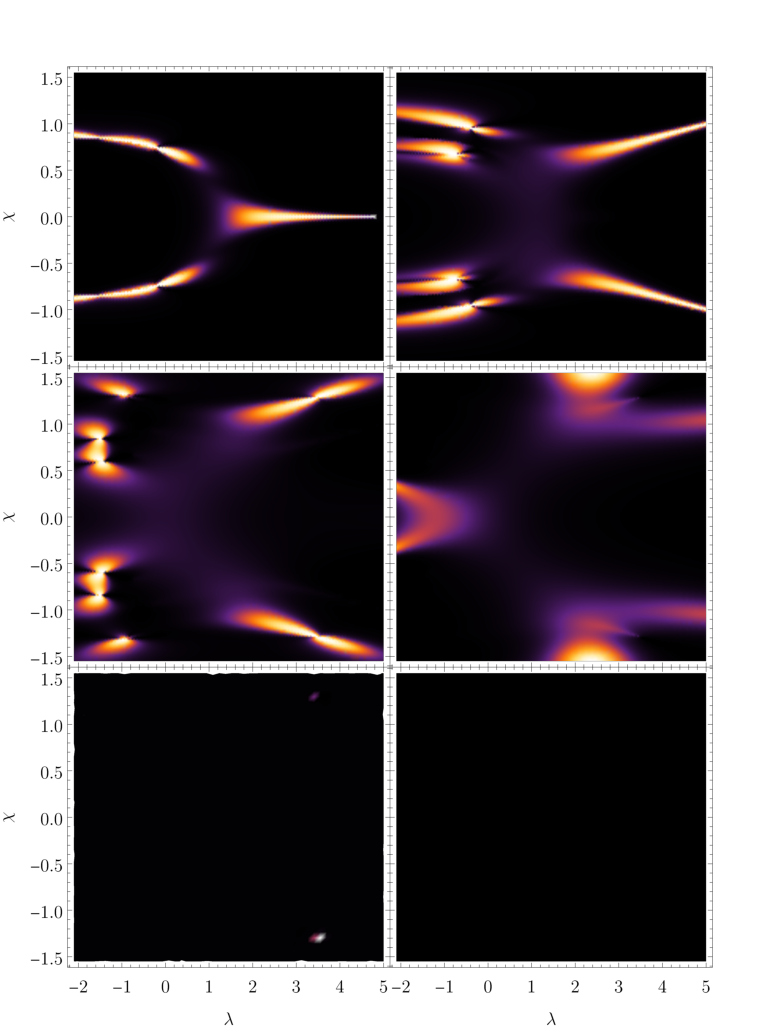
\includegraphics[scale=1.2]{../img/N=5_metricDeterminantElements.pdf}
    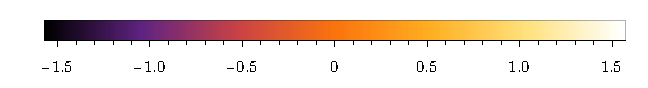
\includegraphics[scale=1.2]{../img/N=3_barA.pdf}
    \caption{Arctangens of the elements of higher state manifolds. By rows using $j$ from the sum in eq. \ref{eq:metrictensorREdefinition}: $j=0$, $j=1$; $j=2$, $j=3$; $j=4$, $j=5$.}
    \label{fig:metricDeterminantElements}    
\end{figure}

\begin{figure}[H]
    \centering
    \includegraphics[scale=1.2]{../img/N=5_metricDeterminants.pdf}
    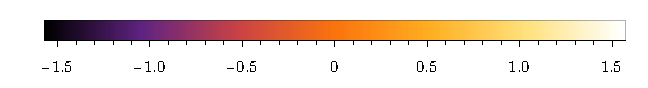
\includegraphics[scale=1.2]{../img/N=3_barA.pdf}
    \caption{Arctangens of the metric tensor for higher state manifolds. By  rows: $M_0$, $M_1$; $M_2$, $M_3$; $M_4$, $M_5$.}
    \label{fig:higherStateManifolds}    
\end{figure}
